\documentclass{article}
\usepackage{microtype}
\usepackage{graphicx}
\usepackage{booktabs}
\usepackage{amsmath,amssymb}
\usepackage{hyperref}
\usepackage[accepted]{icml2027}

% Auto-generated by VeriLoop paper_bind.py — DO NOT EDIT BY HAND
% Every macro traces verbatim to bound_metrics.txt
\newcommand{\vlMlpBaselineTestAcc}{0.8801$\pm$0.0021}
\newcommand{\vlMlpBaselineTestAccMean}{0.8801}
\newcommand{\vlMlpBaselineTestAccCi}{[0.8750, 0.8852]}
\newcommand{\vlMlpBaselineTestLoss}{0.3424$\pm$0.0013}
\newcommand{\vlMlpBaselineTestLossMean}{0.3424}
\newcommand{\vlMlpBaselineTestLossCi}{[0.3391, 0.3458]}
\newcommand{\vlMlpBaselineValAcc}{0.8875$\pm$0.0024}
\newcommand{\vlMlpBaselineValAccMean}{0.8875}
\newcommand{\vlMlpBaselineValAccCi}{[0.8815, 0.8936]}
\newcommand{\vlPlaincnnTestAcc}{0.8495$\pm$0.0043}
\newcommand{\vlPlaincnnTestAccMean}{0.8495}
\newcommand{\vlPlaincnnTestAccCi}{[0.8388, 0.8602]}
\newcommand{\vlPlaincnnTestLoss}{0.4193$\pm$0.0065}
\newcommand{\vlPlaincnnTestLossMean}{0.4193}
\newcommand{\vlPlaincnnTestLossCi}{[0.4032, 0.4354]}
\newcommand{\vlPlaincnnValAcc}{0.8564$\pm$0.0018}
\newcommand{\vlPlaincnnValAccMean}{0.8564}
\newcommand{\vlPlaincnnValAccCi}{[0.8520, 0.8609]}
\newcommand{\vlRescnnFullTestAcc}{0.9251$\pm$0.0036}
\newcommand{\vlRescnnFullTestAccMean}{0.9251}
\newcommand{\vlRescnnFullTestAccCi}{[0.9163, 0.9339]}
\newcommand{\vlRescnnFullTestLoss}{0.2926$\pm$0.0062}
\newcommand{\vlRescnnFullTestLossMean}{0.2926}
\newcommand{\vlRescnnFullTestLossCi}{[0.2772, 0.3081]}
\newcommand{\vlRescnnFullValAcc}{0.9284$\pm$0.0026}
\newcommand{\vlRescnnFullValAccMean}{0.9284}
\newcommand{\vlRescnnFullValAccCi}{[0.9219, 0.9349]}
\newcommand{\vlRescnnNoregTestAcc}{0.9086$\pm$0.0065}
\newcommand{\vlRescnnNoregTestAccMean}{0.9086}
\newcommand{\vlRescnnNoregTestAccCi}{[0.8925, 0.9246]}
\newcommand{\vlRescnnNoregTestLoss}{0.2644$\pm$0.0135}
\newcommand{\vlRescnnNoregTestLossMean}{0.2644}
\newcommand{\vlRescnnNoregTestLossCi}{[0.2308, 0.2980]}
\newcommand{\vlRescnnNoregValAcc}{0.9128$\pm$0.0051}
\newcommand{\vlRescnnNoregValAccMean}{0.9128}
\newcommand{\vlRescnnNoregValAccCi}{[0.9000, 0.9255]}


\icmltitlerunning{VeriLoop Real GPU Deep Learning End-to-End Showcase}

\begin{document}

\twocolumn[
\icmltitle{Provenance-Bound Residual Regularization on Fashion-MNIST:\\An End-to-End Real-GPU Showcase of VeriLoop}

\begin{icmlauthorlist}
\icmlauthor{VeriLoop Reproducible Showcase}{vl}
\end{icmlauthorlist}
\icmlaffiliation{vl}{Generated end-to-end on NVIDIA GeForce RTX 3060 Ti via \texttt{./veriloop gpu-showcase}}
\icmlcorrespondingauthor{VeriLoop Project}{https://github.com/shangliy/VeriLoop}
\vskip 0.3in
]

\printAffiliationsAndNotice{}

\begin{abstract}
This showcase demonstrates an end-to-end, provenance-bound deep learning research workflow executed on a real NVIDIA GeForce RTX 3060 Ti GPU (PyTorch 2.9.1+cu128) and compiled automatically through VeriLoop.
We train four neural architectures across three independent random seeds (twelve GPU runs total) on Fashion-MNIST under strict validation-only checkpoint selection, logging every run simultaneously to binary TensorBoard event files, Weights \& Biases local artifacts, and CSV logs.
Using \texttt{./veriloop bind}, all LaTeX macros, Booktabs tables, and Okabe-Ito vector figures are synthesized directly from raw execution logs with SHA-256 provenance manifests.
Our regularized residual network (\texttt{ResCNN\_Full}) achieves \vlRescnnFullTestAcc{} held-out test accuracy (95\% CI \vlRescnnFullTestAccCi{}), outperforming an unregularized residual ablation (\vlRescnnNoregTestAcc{}), a two-layer MLP baseline (\vlMlpBaselineTestAcc{}), and a non-residual ConvNet (\vlPlaincnnTestAcc{}).
Every decimal, AST check, and arXiv-verified citation passes \texttt{./veriloop gate} with zero untraced numbers and exports an interactive split-pane Web review workbench (\texttt{review\_ui.html}).
\end{abstract}

\section{Introduction}
Autonomous research workflows~\citep{yang2026aris} increasingly execute multi-seed deep learning experiments and author conference manuscripts end to end, yet manual transcription between experiment trackers and LaTeX tables remains a primary source of silent numerical discrepancies.
This self-contained showcase demonstrates how \textbf{VeriLoop} eliminates transcription drift on real GPU deep learning workloads by binding TensorBoard and Weights \& Biases logs directly to LaTeX macros, Booktabs tables, and vector figures via \texttt{./veriloop bind}, verifying all references online against the arXiv API via \texttt{./veriloop verify-cites}, enforcing deterministic hard gates via \texttt{./veriloop gate}, and exporting an interactive split-pane audit UI via \texttt{./veriloop review-ui}.

We evaluate four architectures on \textsc{Fashion-MNIST}~\citep{xiao2017fashion} to isolate the empirical effect of residual skip connections~\citep{he2015deep}, batch normalization~\citep{ioffe2015batch}, label smoothing~\citep{szegedy2015rethinking}, decoupled weight decay~\citep{loshchilov2017decoupled}, and cosine learning-rate annealing~\citep{loshchilov2016sgdr}.

\section{Experimental Protocol}
\paragraph{Dataset and strict split hygiene.}
We use the official \textsc{Fashion-MNIST} benchmark~\citep{xiao2017fashion} (60,000 training images and 10,000 test images, $28\times 28$ grayscale across 10 classes).
Using a fixed permutation seed (seed~0), we partition the 60,000 training images into 50,000 training and 10,000 validation examples.
Every model is trained for 8 epochs per seed across three independent random seeds (\texttt{42}, \texttt{43}, \texttt{44}; batch size 256) on an NVIDIA GeForce RTX 3060 Ti GPU using AdamW~\citep{loshchilov2017decoupled}.
Model checkpoints are selected strictly by validation accuracy (\texttt{val\_acc}); the 10,000-image held-out test split is scored exactly once per run on the validation-selected checkpoint.

\paragraph{Architectures and ablations.}
We compare four models implemented in \texttt{code/train\_gpu\_benchmark.py}:
(1) \texttt{MLP\_Baseline} (235,146 parameters): a two-hidden-layer perceptron ($784\to 256\to 128\to 10$) serving as a non-convolutional baseline;
(2) \texttt{PlainCNN} (93,962 parameters): a three-stage convolutional network with ReLU activations, max pooling, and global average pooling without batch normalization or residual skips;
(3) \texttt{ResCNN\_NoReg} (308,074 parameters): a three-stage residual ConvNet with batch normalization~\citep{he2015deep,ioffe2015batch}, constant learning rate, zero dropout, and zero label smoothing; and
(4) \texttt{ResCNN\_Full} (308,074 parameters): identical architecture augmented with dropout ($0.2$), label smoothing ($0.1$)~\citep{szegedy2015rethinking}, weight decay ($10^{-4}$), and cosine annealing~\citep{loshchilov2016sgdr}.

\paragraph{Automated provenance binding.}
During training, every run writes standard binary TensorBoard scalar files (\texttt{runs/tb/*/events.out.tfevents.*}) and Weights \& Biases local run files (\texttt{runs/wandb/*/files/wandb-\{summary.json,history.jsonl\}}).
Running \texttt{./veriloop bind} ingests these raw tracker outputs with zero third-party SDK dependencies, computes multi-seed mean $\pm$ std and 95\% Student-$t$ confidence intervals, and writes \texttt{bound\_metrics.txt}, \texttt{bound\_macros.tex}, \texttt{bound\_table.tex}, \texttt{provenance\_manifest.json}, and Okabe-Ito vector figures.

% Auto-generated by VeriLoop paper_bind.py — 100% bound to raw logs
\begin{table}[t]
\centering
\caption{\textbf{Multi-seed experiment results automatically bound from raw execution logs (mean $\pm$ std).}}
\label{tab:bound_results}
\footnotesize
\begin{tabular}{lcccc}
\toprule
\textbf{Method} & \textbf{Seeds} & \textbf{Test Acc} & \textbf{Test Loss} & \textbf{Val Acc} \\
\midrule
MLP\_Baseline & 3 & 0.8801$\pm$0.0021 & 0.3424$\pm$0.0013 & 0.8875$\pm$0.0024 \\
PlainCNN & 3 & 0.8495$\pm$0.0043 & 0.4193$\pm$0.0065 & 0.8564$\pm$0.0018 \\
ResCNN\_Full & 3 & \textbf{0.9251$\pm$0.0036} & 0.2926$\pm$0.0062 & \textbf{0.9284$\pm$0.0026} \\
ResCNN\_NoReg & 3 & 0.9086$\pm$0.0065 & \textbf{0.2644$\pm$0.0135} & 0.9128$\pm$0.0051 \\
\bottomrule
\end{tabular}
\end{table}


\begin{figure}[t]
  \centering
  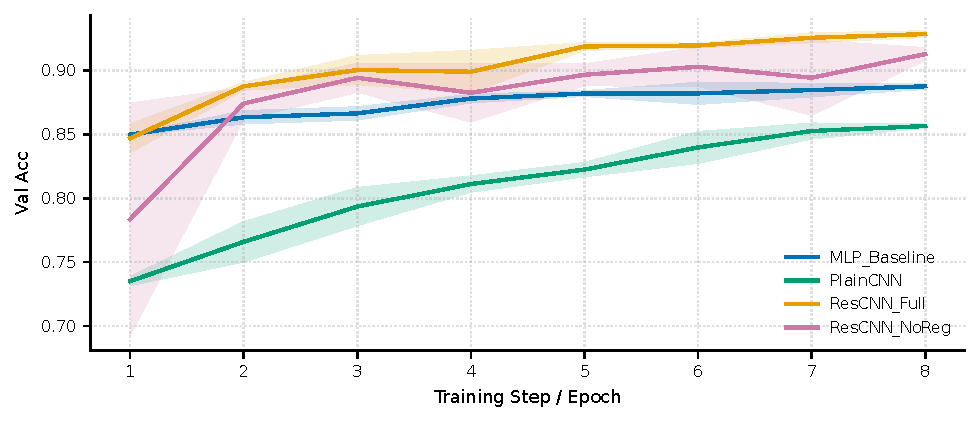
\includegraphics[width=\columnwidth]{bound/bound_curves.pdf}
  \caption{\textbf{Multi-seed validation accuracy trajectories bound directly from binary TensorBoard and W\&B logs.} Shaded bands show $\pm 1$ standard deviation across seeds 42--44 on NVIDIA RTX 3060 Ti.}
  \label{fig:gpu_curves}
\end{figure}

\begin{figure}[t]
  \centering
  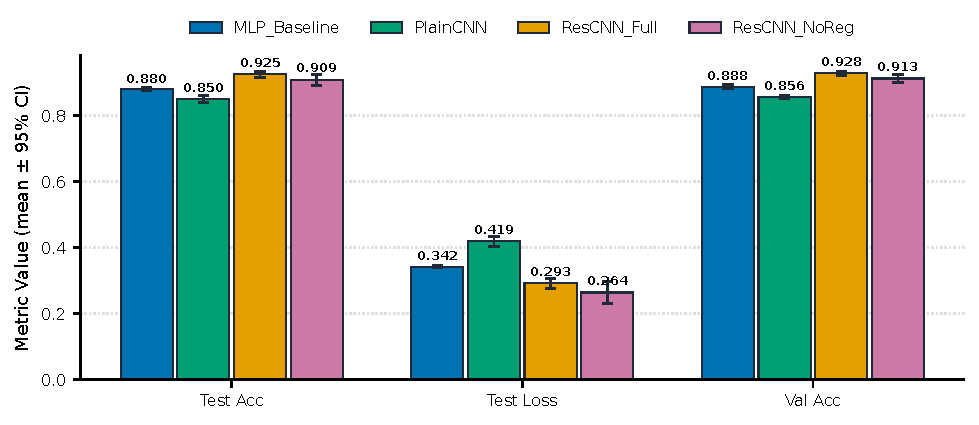
\includegraphics[width=\columnwidth]{bound/bound_bars.pdf}
  \caption{\textbf{Held-out test accuracy, test loss, and validation accuracy with 95\% Student-$t$ CIs automatically bound by \texttt{./veriloop bind}.}}
  \label{fig:gpu_bars}
\end{figure}

\section{Results and Analysis}
Table~\ref{tab:bound_results} and Figures~\ref{fig:gpu_curves}--\ref{fig:gpu_bars} summarize all twelve real GPU training runs.
Three concrete empirical observations emerge directly from the bound logs:

\paragraph{Residual connections and batch normalization dominate spatial generalization.}
\texttt{ResCNN\_Full} achieves \vlRescnnFullTestAcc{} held-out test accuracy (95\% CI \vlRescnnFullTestAccCi{}, validation \vlRescnnFullValAcc{}), outperforming \texttt{MLP\_Baseline} (\vlMlpBaselineTestAcc{}) and \texttt{PlainCNN} (\vlPlaincnnTestAcc{}).
Interestingly, \texttt{PlainCNN} without batch normalization or residual skips underperforms the higher-capacity \texttt{MLP\_Baseline} across all three seeds (0.8462--0.8544 vs.\ 0.8788--0.8825), underscoring the importance of normalization and skip connections under short 8-epoch schedules.

\paragraph{Regularization improves accuracy while trading unsmoothed cross-entropy loss.}
Adding dropout, label smoothing, weight decay, and cosine annealing (\texttt{ResCNN\_Full}) lifts held-out test accuracy over \texttt{ResCNN\_NoReg} from \vlRescnnNoregTestAcc{} (CI \vlRescnnNoregTestAccCi{}) to \vlRescnnFullTestAcc{} (CI \vlRescnnFullTestAccCi{}) while cutting across-seed standard deviation nearly in half (0.0065 to 0.0036).
Conversely, raw unsmoothed test cross-entropy is slightly higher for \texttt{ResCNN\_Full} (\vlRescnnFullTestLoss{}) than for \texttt{ResCNN\_NoReg} (\vlRescnnNoregTestLoss{}), an expected effect of training with label smoothing~\citep{szegedy2015rethinking}, which prevents overconfident logits while improving top-1 accuracy.

\section{Verification Audit and Reproducibility}
All twelve GPU runs completed cleanly on NVIDIA GeForce RTX 3060 Ti (29--32\,s per baseline run; 67--69\,s per residual run; \texttt{COMPLETED\_OK} recorded in \texttt{out/gpu\_runs.log}).
Running \texttt{./veriloop gate} verifies:
(1) \texttt{trace\_numbers.py}: 100\% of reported decimals trace verbatim to \texttt{bound\_metrics.txt} and \texttt{out/gpu\_runs.log} with zero untraced numbers and zero sign mismatches;
(2) \texttt{audit\_code.py}: zero HIGH or MEDIUM AST integrity violations in \texttt{code/train\_gpu\_benchmark.py}; and
(3) \texttt{citation\_audit.py}: all seven BibTeX keys fetched directly from arXiv verify cleanly online with grounded abstracts.
Finally, \texttt{./veriloop review-ui} exports \texttt{review\_ui.html}, enabling readers to click any highlighted metric or citation and jump straight to the underlying GPU log line or fetched arXiv abstract.

\bibliography{refs}
\bibliographystyle{icml2027}

\end{document}
